\section{Coresets and Sensitivity Sampling}

In this work, we are using the method of coresets
(see for example~\cite{munteanu-coresets-introduction})
to approach the problem of data reduction for the probit model.
The idea behind coresets is, that when given a
dataset $\mathcal{D}$, we are interested in selecting
only a small subset of observations
$\mathcal{C} \subseteq \mathcal{D}$, such that the objective
function evaluated on the (possible reweighted) subset $\mathcal{C}$
does not differ too much
from the objective function evaluated on the original dataset $\mathcal{D}$.

This approach will allow us to estimate the model parameters
efficiently on the ideally much smaller set $\mathcal{C}$,
when a full optimization on $\mathcal{D}$ could already
be infeasible for big datasets.
We are thus following the paradigm of \textit{sketch-and-solve},
i.e. first reducing the size of the original dataset and then solving
the optimization problem on the reduced dataset.

In order to work out a formal definition of when we call a subset
$\mathcal{C} \subseteq \mathcal{D}$ a coreset in the context of
probit regression, we first have to slightly extend the
concept of the model matrix, as we will need it for the coreset
definition.

\begin{definition}[Scaled model matrix]
    Let $\mathcal{D}=\{(x_i, y_i)\}_{i=1}^n$ be a $d$-dimensional dataset.
    Let $z_i = (2y_i - 1)x_i$ for all i in $[n]$.
    Then we call the matrix $Z \in \mathbb{R}^{n \times d}$, where the
    $i$-th row consists of the vector $z_i$ for all $i \in [n]$,
    the scaled model matrix of $\mathcal{D}$.
\end{definition}

This definition of the scaled model matrix is nothing particularly new,
it just formalizes the concept of factoring the labels into the
model matrix, which we already encountered when dealing with the
parameter estimation in section~\ref{sec:parameter-estimation}.

We are now ready for the coreset definition:

\begin{definition}[Coreset]
    \label{def:coreset}
    Let $\mathcal{D}=\{(x_i, y_i)\}_{i=1}^n$ be a $d$-dimensional dataset
    with scaled model matrix $Z \in \mathbb{R}^{n \times d}$ and
    a vector of positive sample weights $w \in \mathbb{R}_{>0}^n$.
    Let $\mathcal{C} \subseteq \mathcal{D}$ be a subset of $\mathcal{D}$
    of size $|\mathcal{C}| = k$
    with scaled model matrix $C \in \mathbb{R}^{k \times d}$ and
    a vector of positive sample weights $u \in \mathbb{R}_{>0}^k$.
    Let $\frac{1}{2} > \epsilon > 0$.
    We call $\mathcal{C}$ a $(1+\epsilon)$-coreset of $\mathcal{D}$
    for probit regression, if
    \begin{equation*}
        (1-\epsilon)f_Z^w(\beta) \leq f_C^u(\beta) \leq (1+\epsilon)f_Z^w(\beta)
        \quad \forall \beta \in \mathbb{R}^d,
    \end{equation*}
    where $f_Z^w(\beta) = \sum_{i=1}^n w_i g(z_i^T \beta)$ is the
    weighted objective function of the probit model.
\end{definition}

The size parameter $k = |\mathcal{C}|$ of a coreset usually depends
on the desired approximation quality $\epsilon$, as well as on
specific problem characteristics, such as the number of observations
$n$ as well as the dimensionality $d$ of the dataset.
When constructing coresets, we are interested in keeping this parameter
low in comparison to the total size of the dataset, i.e. we
usually require that at least $k \in O(\log{n})$, so that
the data reduction is actually meaningful.

In the next section, we will investigate if there are any
guarantees that can be given regarding the coreset size
without imposing any further restrictions on the dataset.
We will find out, that in the general case, it can't
be guaranteed that a reasonably small coreset always exists.
As a consequence, we will later confine our research to a
specific class of datasets that we will call $\mu$-complex,
for which small upper bounds on the coreset size can be
derived.

\subsection{Lower Bounds for Coreset Size in the General Case}

The first result that we will take a look at in the following
theorem shows, that there are some datasets, for which
no sufficiently small coresets of a size of at maximum $k \in O(\log n)$
can be found.

\begin{theorem}
    \label{theorem:index}
    There exists a $d$-dimensional dataset $\mathcal{D}$ of size
    $|\mathcal{D}| = n$, such
    that any $(1+\epsilon)$-coreset $\mathcal{C}$ of $\mathcal{D}$
    for probit regression has a size $k = |\mathcal{C}|$
    of at least $k \in \Omega\left(\frac{n}{\log{n}}\right)$.
\end{theorem}
\begin{proof}
    We can construct such a  dataset by showing
    how coresets can be used in a
    communication protocol for the so called INDEX communication game
    to encode a message.
    Since there exists a lower bound on the minimum
    message length of the INDEX game (see~\cite{index}),
    we can use it to derive a lower bound on the
    coreset size.
    The same technique was also used in~\cite{on-coresets} to find
    lower bounds for coresets of logistic regression and is here slightly
    adapted for probit regression.

    The INDEX game consists of two players, Alice and Bob.
    Alice is given a random binary string $m \in \{0, 1\}^n$ of $n$ bits
    and Bob is given an index $i \in [n]$.
    The goal is for Alice to send a message to Bob that allows
    Bob to obtain the value $m_i$ of Alice's binary string $m$.
    It was shown in~\cite{index}, that the minimum length of a message
    sent by Alice that still allows Bob to obtain $m_i$ with
    constant probability is in $\Omega(n)$ bits.
    We will now see how a coreset for probit regression can be used
    to encode such a message.

    The first step is for Alice to convert her binary string $m$ into
    a two-dimensional dataset $\mathcal{D}$ as follows:
    For each entry $m_j$ of her binary string where $m_j = 1$, she adds
    a point
    \begin{equation*}
        x_j = \left( \cos{\left(2 \pi \frac{j}{n}\right)},
        \sin{\left(2 \pi \frac{j}{n}\right)} \right)^T
    \end{equation*}
    to her set $\mathcal{D}$ and labels it with $y_j = 1$,
    ending up with the dataset
    \begin{equation*}
        \mathcal{D} = \{(x_j, 1)\}_{j \in \{i \in [n]:\ m_i = 1 \}}.
    \end{equation*}
    As we can see, all of these points are on the unit circle and all
    of them are labeled with $1$.

    The next step for her is to construct a
    $(1+\epsilon)$-coreset $\mathcal{C}$ of $\mathcal{D}$
    for probit regression with sample weights $u \in \mathbb{R}^k_{>0}$
    and to transmit both the coreset and the weight vector to Bob.
    We will later see, how
    large the size $|\mathcal{C}|=k$ of this coreset must be,
    so that Bob can still
    obtain the value of $m_i$ with constant probability.

    As soon as Alice's coreset $\mathcal{C}$ arrives at Bob,
    Bob can use it to obtain the value of $m_i$.
    To do this, Bob first adds two new points
    \begin{equation*}
        q_1 = \left( \cos{\left(2 \pi \frac{i - 0.5}{n}\right)},
        \sin{\left(2 \pi \frac{i - 0.5}{n}\right)} \right)^T
    \end{equation*}
    and
    \begin{equation*}
        q_2 = \left( \cos{\left(2 \pi \frac{i + 0.5}{n}\right)},
        \sin{\left(2 \pi \frac{i + 0.5}{n}\right)} \right)^T
    \end{equation*}
    to the set and labels both points with $0$ (see figure~\ref{fig:index}),
    i.e. Bob now has the dataset
    \begin{equation*}
        \mathcal{C}' = \mathcal{C} \cup \{(q_1, 0)\} \cup \{(q_2, 0)\}.
    \end{equation*}

    Next, he uses this new dataset $\mathcal{C}'$ with
    scaled model matrix $C'$ to
    minimize the weighted objective function
    $f_{C'}^u$ of the probit model,
    by using the Newton-Raphson optimization algorithm.

    Taking a look at figure~\ref{fig:index}, it becomes evident,
    that Bobs points $q_1$ and $q_2$ are linearly separable from
    the other points if and only if Alice didn't add a point
    $x_i$, i.e. if $m_i = 0$.
    He can use the results of the optimization procedure to
    make a distinction between the two cases
    (which then allows him to determine the value of $m_i$)
    like this:

    In the case of $m_i=1$, Bobs points are not linearly separable from
    Alices points, which means that there must occur at least one
    misclassification at a cost of $g(0) = \log(2)$.
    Because Bobs dataset $\mathcal{C}'$ allows him to obtain a
    $(1 \pm \epsilon)$-approximation of the cost function, he can
    check if the Newton-Raphson algorithm converges to
    a cost of at least $(1 - \epsilon) \log(2) \geq \frac{1}{2} \log(2)$.
    In this case, he knows that Alice must have added the point $x_i$,
    which means that $m_i=1$.

    Conversely, if at any point during the optimization procedure
    the cost function drops below
    $\frac{1}{2} \log(2)$
    and approaches zero, Bob knows that Alice didn't add the point
    $x_i$, because his dataset $\mathcal{C}'$ is linearly separable.
    This will allow him to conclude that $m_i = 0$.

    % There is one special case that has to be dealt with in order for this
    % protocol to work. If Alice's coreset $\mathcal{C}$
    % only consists of the single point
    % $x_i$, Bob's points $q_1$ and $q_2$ could still be linearly seperated
    % although Alice added $x_i$.
    % The workaround to this is simple though:
    % Bob can always just add two more
    % points at the locations of $x_{i-1}$ and $x_{i+1}$ and label them with 1.
    % Now, $q_1$ and $q_2$ can only be linearly seperated from the
    % other points if and only if Alice didn't add a point $x_i$.

    Let us now see how big the size $k$ of Alice's coreset must be
    for this protocol to work with constant probability.
    In~\cite{index} it was shown, that the minimum length of a message
    that Alice must send in order for the protocol to work
    is in $\Omega(n)$ bits.
    Since each of the points that Alice created can be encoded in
    $\log(n)$ space, it follows from the lower bound that
    $\Omega(n) \subseteq \Omega(k \log(n))$, so $k$ must be in
    $\Omega\left(\frac{n}{\log(n)}\right)$.

    We can conclude, that if there existed a $(1 + \epsilon)$-coreset
    of $\mathcal{D}$
    for probit regression with size $k \in o\left(\frac{n}{\log(n)}\right)$,
    it would contradict the minimum message length of
    the INDEX communication game, which proves the theorem.
\end{proof}

\begin{figure}[h]
    \centering
    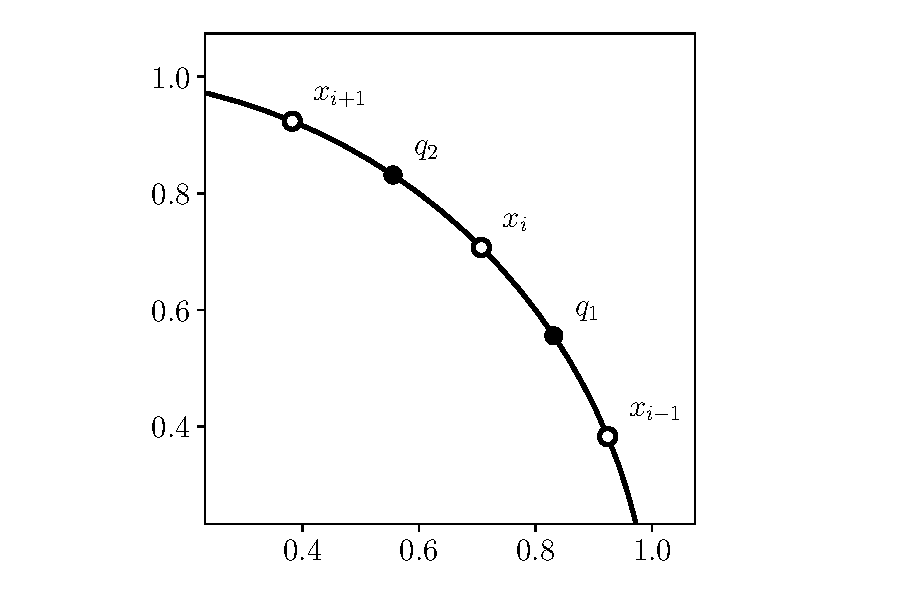
\includegraphics[width=0.8\textwidth]{figures/index.pdf}
    \caption{Bob places two points $q_1$ and $q_2$ in such a way
        on the unit circle, that they can be linearly seperated from the other
        points if and only if Alice didn't place a point at $x_i$.}
    \label{fig:index}
\end{figure}

In the proof of theorem~\ref{theorem:index}, we have already encountered
such a "degenerate" dataset, for which no sublinear sized coreset can be found,
consisting of only positive labels.
The next step of this work is to introduce a new complexity measure
for datasets in the context of probit regression, that allows us
to specify a broad class of datasets for which sublinear sized
coresets do exist and to show how such coresets can be constructed
for this class.
The idea behind this complexity measure goes back to
the work in~\cite{on-coresets}, where the authors introduced a similar
measure to describe a class of datasets that allow the construction
of sublinear coresets in the context of logistic regression.
We adapt this measure to the context of probit regression in the
following definition.

\begin{definition}($\mu$-complexity)
    \label{def:mu}
    Let $\mathcal{D}$ be a $d$-dimensional dataset of size
    $|\mathcal{D}|=n$ with scaled
    model matrix $Z \in \mathbb{R}^{n \times d}$, where
    $z_i \in \mathbb{R}^d$ constitutes the $i$-th
    row of $Z$ and let
    $w \in \mathbb{R}^n_{>0}$ be a vector of positive weights.
    Let $I_\beta^+ = \{i \in [n]:\ w_i z_i^T \beta > 0 \}$
    and let $I_\beta^- = \{i \in [n]:\ w_i z_i^T \beta < 0 \}$.
    Let
    \begin{equation*}
        \mu_w(\mathcal{D}) = \sup_{\beta \in \mathbb{R}^d \setminus \{0\}}
        \frac{\sum_{i \in I_\beta^+} w_i (z_i^T \beta)^2}
        {\sum_{i \in I_\beta^-} w_i (z_i^T \beta)^2}.
    \end{equation*}
    We call the dataset $\mathcal{D}$ with weight vector $w$
    $\mu$-complex, if there exists a $\mu \in \mathbb{R}$,
    such that $\mu_w(\mathcal{D}) \leq \mu$.
\end{definition}

There is a close relationship between $\mu$ and the linear
separability of a dataset as shown in the following theorem.

\begin{theorem}
    \label{theorem:mu-linear-separability}
    Let $\mathcal{D}$ be a $d$-dimensional dataset of size
    $|\mathcal{D}| = n$ like in definition~\ref{def:mu}
    and let $w \in \mathbb{R}^n_{>0}$ be a vector of
    positive weights.
    Then, the dataset
    $\mathcal{D}$ with weight vector $w$ is $\mu$-complex
    if and only if $\mathcal{D}$ is not linearly separable.
\end{theorem}
\begin{proof}
    We first prove the "$\Rightarrow$" direction, i.e. we show
    that if $\mathcal{D}$ is $\mu$-complex,
    then it is not linearly separable.
    We do this by proving the equivalent
    contraposition that if $\mathcal{D}$ is linearly separable,
    then it is not $\mu$-complex.

    Let $S_0 = \{i \in [n]:\ y_i = 0\}$ and $S_1 = \{i \in [n]:\ y_i = 1\}$
    like in definition~\ref{def:linear-separability}.
    If $\mathcal{D}$ is linearly separable, then there exists
    a $\beta \in \mathbb{R}^d \setminus \{0\}$, such that
    \begin{align*}
                    & \forall i \in S_0:\ x_i^T \beta \leq 0\quad \text{and}\quad \forall i \in S_1:\ x_i^T \beta \geq 0                       \\
        \iff        &                                                                                                                          \\
                    & \forall i \in S_0:\ (-1) x_i^T \beta \geq 0\quad \text{and}\quad \forall i \in S_1:\ x_i^T \beta \geq 0                  \\
        \iff        &                                                                                                                          \\
                    & \forall i \in S_0:\ (2y_i - 1) x_i^T \beta \geq 0\quad \text{and}\quad \forall i \in S_1:\ (2y_i - 1) x_i^T \beta \geq 0 \\
        \iff        &                                                                                                                          \\
                    & \forall i \in S_0:\ z_i^T \beta \geq 0\quad \text{and}\quad \forall i \in S_1:\ z_i^T \beta \geq 0                       \\
        \iff        &                                                                                                                          \\
                    & \forall i \in [n]:\ z_i^T\beta \geq 0                                                                                    \\
        \iff        &                                                                                                                          \\
                    & I_\beta^- = \{ i \in [n]:\ w_iz_i^T\beta < 0\} = \emptyset                                                               \\
        \iff        &                                                                                                                          \\
                    & \sum_{i \in I_\beta^-} w_i (z_i^T \beta)^2 = 0                                                                           \\
        \Rightarrow &                                                                                                                          \\
                    & \mu_w(\mathcal{D}) \geq \frac{\sum_{i \in I_\beta^+} w_i (z_i^T \beta)^2}
        {\sum_{i \in I_\beta^-} w_i (z_i^T \beta)^2} = \infty,
    \end{align*}
    which means that $\mathcal{D}$ is not $\mu$-complex.

    It now remains to prove the "$\Leftarrow$" direction, i.e. to
    show that if $\mathcal{D}$ is not linearly separable,
    then it is $\mu$-complex. Again, we do this by proving the
    equivalent contraposition that if $\mathcal{D}$ is not
    $\mu$-complex, then it is linearly separable.

    The first step in order to do so is to show that we can restrict the
    supremum in $\mu_w(\mathcal{D})$ to finite $\beta$ with
    $\lVert \beta \rVert = 1$:
    \begin{align*}
        \mu_w(\mathcal{D}) & = \sup_{\beta \in \mathbb{R}^d \setminus \{0\}}
        \frac{\sum_{i \in I_\beta^+} w_i (z_i^T \beta)^2}
        {\sum_{i \in I_\beta^-} w_i (z_i^T \beta)^2}                                         \\ & =
        \sup_{\beta \in \mathbb{R}^d \setminus \{0\}}
        \frac{\sum_{i \in I_\beta^+} \frac{1}{\lVert \beta \rVert^2}w_i (z_i^T \beta)^2}
        {\sum_{i \in I_\beta^-} \frac{1}{\lVert \beta \rVert^2} w_i (z_i^T \beta)^2}         \\
                           & =
        \sup_{\beta \in \mathbb{R}^d \setminus \{0\}}
        \frac{\sum_{i \in I_\beta^+} w_i \left(z_i^T \frac{\beta}{\lVert \beta \rVert}\right)^2}
        {\sum_{i \in I_\beta^-}  w_i \left(z_i^T \frac{\beta}{\lVert \beta \rVert}\right)^2} \\
                           & =
        \sup_{\tilde\beta \in \mathbb{R}^d,\ \lVert \tilde\beta \rVert = 1}
        \frac{\sum_{i \in I_\beta^+} w_i \left(z_i^T \tilde\beta \right)^2}
        {\sum_{i \in I_\beta^-}  w_i \left(z_i^T \tilde\beta \right)^2},
    \end{align*}
    which lets us conclude that even in the supremum, both expressions
    $\sum_{i \in I_\beta^+} w_i (z_i^T \beta )^2$
    and
    $\sum_{i \in I_\beta^-}  w_i (z_i^T \beta )^2$
    are finite.
    This means that if $\mathcal{D}$ is not $\mu$-complex, then
    the denominator must be zero, i.e. it must hold that there exists
    a $\beta \in \mathbb{R}^d \setminus \{0\}$ such that
    \begin{equation*}
        \sum_{i \in I_\beta^-}  w_i (z_i^T \beta )^2 = 0.
    \end{equation*}

    From here, we can follow the same chain of equivalences that we
    showed when proving the "$\Rightarrow$"-direction of the theorem,
    which leads us directly to the fact, that $\mathcal{D}$ in this case must
    be linearly separable, which concludes the proof.
\end{proof}

As we already noted in section~\ref{sec:parameter-estimation},
linear separability is also closely related to the existence
of the maximum likelihood estimate in the probit model.
The next theorem uses the relationship between $\mu$ and
linear separability to show the connection between $\mu$
and the existence and uniqueness of the maximum likelihood estimate.

\begin{theorem}
    Let $\mathcal{D}$ be a $d$-dimensional dataset of size
    $|\mathcal{D}| = n$ with model matrix $X \in \mathbb{R}^{n \times d}$
    and $rank(X) = d$, i.e. $X$ has full column rank.
    Then, the maximum likelihood estimate $\tilde\beta$ for the probit
    model exists and is unique if and only if $\mathcal{D}$ is $\mu$-complex.
\end{theorem}
\begin{proof}
    This is a direct corollary from theorem~\ref{theorem:probit-existence}
    and theorem~\ref{theorem:mu-linear-separability}.
    For model matrices with full column rank, the uniqueness of the
    MLE follows
    direclty from its existence, as shown in~\cite{wedderburn}.
\end{proof}

In the following parts of this work, we will derive efficient upper
bounds on the coreset size for $\mu$-complex datasets.
In order to do this, we first introduce a theoretic
framework that we use for the coreset construction which
is based on the concept of sensitivities.

\subsection{The Sensitivity Framework}

The sensitivity framework, which was first introduced
by~\cite{feldman-langberg-coresets} (see also
\cite{big-data-tiny-data} for a detailed overview),
is a method for constructing
provably small coresets by randomly sampling observations
from a dataset according to a probability distribution, that
emphasizes observations, which have a greater impact on the
objective function.

Instead of representing a dataset $\mathcal{D} = \{(x_i, y_i)\}_{i=1}^n$
as a set of labeled datapoints, the sensitivity framework
represents each point as a function that describes its
contribution to the objective function.
Recall, that in~\ref{sec:parameter-estimation}, we defined the
weighted objective function of the probit model as
$f_Z^w(\beta) = \sum_{i=1}^n w_i g(z_i^T \beta)$.
We will now associate each datapoint $(x_i, y_i)$ with the function
$g_i(\beta) := g(z_i^T \beta) = g((2y_i - 1)x_i^T \beta)$,
that describes its contribution to the total loss.
That way, we can equivalently represent a dataset in the context
of probit regression as a collection of loss functions
$F = \{g_1, ..., g_n\}$.

The idea behind the sensitivity framework is to draw a random
sample from this set of functions, where the sampling probability
of each function is proportional to its worst-case
contribution to the total loss for any $\beta \in \mathbb{R}^d$.
This worst-case importance is also called sensitivity and was first
introduced in~\cite{langberg-schulman-sensitivities}:

\begin{definition}[\cite{langberg-schulman-sensitivities}]
    \label{def:sensitivity}
    Let $F = \{ g_1, ..., g_n \}$ be a set of functions,
    $g_i: \mathbb{R}^d \rightarrow \mathbb{R}_{\geq 0}, \ i \in [n]$
    and let $w \in \mathbb{R}^n_{>0}$ be a vector of positive weights.
    The sensitivity of $g_i$ for $f_w(\beta) = \sum_{i=1}^n w_i g_i(\beta)$ is defined as
    \begin{equation*}
        \varsigma_i = \sup_{\beta \in \mathbb{R}^d, \ f_w(\beta) > 0} \frac{w_i g_i(\beta)}{f_w(\beta)}.
    \end{equation*}
    The total sensitivity, i.e. the sum of the sensitivities is $\mathfrak{S} = \sum_{i=1}^n \varsigma_i$.
\end{definition}

The true sensitivity $\varsigma_i$ of a function $g_i$ is usually unknown
and its computation can be expensive, because it involves solving the
original optimization problem, which was indicated in~\cite{braverman-feldman-coresets}.
For this reason, we are usually interested to find efficiently computable
upper bounds $s_i \geq \varsigma_i$ for the sensitivities and then
to draw samples proportional to the upper bounds $s_i$.
As we will see, as long as the sum $S = \sum_{i=1}^n s_i$ of the upper
bounds is sufficiently small, the coreset size will be small as well.

The second element of the sensitivity framework, which
\cite{feldman-langberg-coresets} related to the
concept of sensitivity sampling in order to obtain small coresets,
is the theory of range spaces and the VC-dimension.
Its relevant definitions are given below.

\begin{definition}[\cite{feldman-langberg-coresets}]
    A range space is a pair $\mathfrak{R} = (F, \textup{ranges})$, where F is a set
    and $\textup{ranges}$ is a family (set) of subsets of F.
\end{definition}

\begin{definition}[\cite{feldman-langberg-coresets}]
    The VC-dimension $\Delta(\mathfrak{R})$ of a range space
    $\mathfrak{R} = (F, \textup{ranges})$ is
    the size $|G|$ of the largest subset $G \subseteq F$ such that
    \begin{equation*}
        \left| \left\{ G \cap R \ | \ R \in \textup{ranges} \right\} \right|
        = 2^{|G|},
    \end{equation*}
    i.e. $G$ is shattered by $\textup{ranges}$.
\end{definition}

\begin{definition}[\cite{feldman-langberg-coresets}]
    Let $F$ be a finite set of functions mapping from $\mathbb{R}^d$ to $\mathbb{R}^{\geq 0}$.
    For every $\beta \in \mathbb{R}^d$ and $r \geq 0$, let
    \begin{equation*}
        \textup{range}(F, \beta, r) = \left\{ f \in F \ | \  f(\beta) \geq r  \right\}
    \end{equation*}
    and let
    \begin{equation*}
        \textup{ranges}(F) = \left\{ \textup{range}(F, \beta, r) \ | \ \beta \in \mathbb{R}^d, \ r \geq 0  \right\}.
    \end{equation*}
    Then we call $\mathfrak{R}_F := (F, \textup{ranges}(F))$ the range space induced by F.
\end{definition}

The following theorem is the basis of the sensitivity framework and
combines the theory of range spaces with the concept of
sensitivity sampling. Its original version goes back to
\cite{feldman-langberg-coresets}, but it was
further improved by
\cite{braverman-feldman-coresets}.
In this work, we will use the following variant by~\cite{big-data-tiny-data}:

\begin{theorem}[\cite{big-data-tiny-data}]
    \label{theorem:sensitivity-framework}
    Let $F = \{ g_1, ..., g_n \}$ be a set of functions,
    $g_i: \mathbb{R}^d \rightarrow \mathbb{R}_{\geq 0}, \ i \in [n]$
    and let $w \in \mathbb{R}^n_{>0}$ be a vector of positive weights.
    Let $\epsilon, \delta \in (0, \frac{1}{2})$.
    Let $s_i \geq \varsigma_i$ be upper bounds of the sensitivities and
    let $S = \sum_{i=1}^n s_i$.
    Given $s_i$, one can compute in time $O(|F|)$ a set
    $R \subseteq F$ of
    \begin{equation*}
        |R| \in O \left( \frac{S}{\epsilon^2} \left( \Delta \log S + \log \left( \frac{1}{\delta} \right) \right) \right)
    \end{equation*}
    weighted functions, such that with probability $1 - \delta$ we have
    for all $\beta \in \mathbb{R}^d$ simultaneously
    \begin{equation*}
        (1-\epsilon) \sum_{g_i \in F} w_i g_i(\beta) \leq \sum_{g_i \in R} u_i g_i(\beta) \leq (1 + \epsilon) \sum_{g_i \in F} w_i g_i(\beta).
    \end{equation*}
    Each element of $R$ is sampled independently with probability
    $p_j = \frac{s_j}{S}$ from $F$, $u_i = \frac{S w_j}{s_j |R|}$
    denotes the weight of a function $g_i \in R$ that corresponds to
    $g_j \in F$ and $\Delta$ is an upper bound on the
    VC-dimension of the range space $\mathfrak{R}_{F^\ast}$ induced by
    $F^\ast$, where $F^\ast$ is the set of functions $g_i \in F$
    scaled by $\frac{S w_i}{s_i |R|}$, i.e.
    $F^\ast = \left\{ \frac{S w_i}{s_i |R|} g_i(\beta) \ |\ i \in [n] \right\}$.
\end{theorem}

From this theorem, it follows that there are two things that have to be
done in order to find a small coreset for probit regression.

The first one is to find small and efficiently computable upper bounds
on the sensitivities and the second thing is to find a
small upper bound on the VC-dimension of the range space induced by $F^\ast$.
We will do both in the following section.

\subsection{Constructing the Coreset}

\subsubsection{Bounding the Sensitivity}

The first thing we need to do in order to find upper bounds on
the sensitivities is to find bounds on the function $g$,
which we do in the following two lemmas.

\begin{lemma}
    Let $g(x) = \ln \left( \frac{1}{1 - \Phi(x)}\right)$.
    Then, for all $x \geq 0$, it holds that:
    \begin{equation*}
        \frac{1}{2} x^2 \leq g(x).
    \end{equation*}
\end{lemma}
\begin{proof}
    We first show the claim for all $x \geq 1$, by using the following
    inequality:
    \begin{align*}
        \Phi(-x) & = \frac{1}{\sqrt{2 \pi}} \int_{-\infty}^{-x} \exp{ \left(-\frac{1}{2} z^2 \right)} dz       \\
                 & \leq \frac{1}{\sqrt{2 \pi}} \int_{-\infty}^{-x} -z \exp{ \left(-\frac{1}{2} z^2 \right)} dz \\
                 & = \frac{1}{\sqrt{2 \pi}} \exp{\left( -\frac{1}{2} x^2 \right)}                              \\
                 & \leq \exp{\left( -\frac{1}{2} x^2 \right)}.                                                 \\
    \end{align*}
    In the next step, we use this inequality to show that for $x \geq 1$:
    \begin{gather*}
        e^{g(x)} = e^{\ln \left( \frac{1}{1 - \Phi(x)} \right)} = \frac{1}{\Phi(-x)} \geq e^{\frac{1}{2} x^2}\\
        \iff \\
        g(x) \geq \frac{1}{2} x^2,
    \end{gather*}
    which proves the theorem for $x \geq 1$.

    Let us now turn to the case when $0 \leq x \leq 1$.
    Both $g(x)$ and $\frac{1}{2}x^2$ are monotonically increasing
    and continuous functions for $0 \leq x \leq 1$.
    Making use of the fact that $g(0) > \frac{1}{2}$, it follows
    for all $0 \leq x \leq 1$, that
    \begin{equation*}
        g(x) \geq g(0) > \frac{1}{2} = \max_{0 \leq x \leq 1} \frac{1}{2} x^2 \geq \frac{1}{2} x^2,
    \end{equation*}
    which concludes the proof.
\end{proof}

\begin{lemma}
    Let $g(x) = \ln \frac{1}{1 - \Phi(x)}$.
    Then, for all $x \geq 2$, it holds that:
    \begin{equation*}
        g(x) \leq x^2.
    \end{equation*}
\end{lemma}
\begin{proof}
    In~\cite{gaussian_bounds}, it was shown that the following inequality
    holds for all $x \geq 0$:
    \begin{equation*}
        \Phi(-x) \geq \frac{1}{\sqrt{2 \pi}} \frac{x}{x^2 + 1} e^{-\frac{1}{2} x^2}.
    \end{equation*}
    We can use this equality to establish that for all
    $x \geq 2$ it holds that:
    \begin{align*}
        e^{x^2} \cdot \Phi(-x) & \geq e^{x^2} \frac{1}{\sqrt{2 \pi}} \frac{x}{x^2 + 1} e^{-\frac{1}{2} x^2}                           \\
                               & = e^{\frac{1}{2} x^2} \frac{1}{\sqrt{2 \pi}} \frac{x}{x^2 + 1}                                       \\
                               & = e^{\frac{1}{2} x^2} \frac{1}{\frac{4}{3}\left( x^2 + 1 \right)} \frac{\frac{4}{3} x}{\sqrt{2 \pi}} \\
                               & \geq \frac{e^{\frac{1}{2} x^2}}{\frac{4}{3}\left( x^2 + 1 \right)}                                   \\
                               & \geq \frac{e^{\frac{1}{2} x^2}}{e^{\frac{1}{2} x^2}}                                                 \\
                               & = 1                                                                                                  \\
        \iff                                                                                                                          \\
        e^{x^2}                & \geq \frac{1}{1 - \Phi(x)}                                                                           \\
        \iff                                                                                                                          \\
        x^2                    & \geq \ln \left(\frac{1}{1 - \Phi(x)}\right) = g(x),
    \end{align*}
    which completes the proof.
\end{proof}

\begin{lemma}
    Let $\mathcal{D}$ be a $d$-dimensional and $\mu$-complex dataset of size
    $|\mathcal{D}|=n$ with scaled model matrix
    $Z \in \mathbb{R}^{n \times d}$ and let $w \in \mathbb{R}^d_{>0}$
    be a vector of positive weights.
    Let $F = \{g_1, ..., g_n\}$ be a set of functions with
    $g_i(\beta) = g(z_i^T \beta)$ and let
    $f_w(\beta) = \sum_{i=1}^n w_ig_i(\beta)$.
    Then, it holds that
    \begin{equation*}
        w_jg_j(\beta) \leq 2 \lVert U_j \rVert_2^2(1 + \mu)f_w(\beta) \quad
        \forall\ j \in \{i \in [n]:\ z_i^T \beta \geq 2 \},
    \end{equation*}
    where $U \in \mathbb{R}^{n \times d}$ is an orthonormal basis for
    the columnspace of $\sqrt{D_w}Z$ and $\sqrt{D_w} \in \mathbb{R}^{n \times n}$
    is a diagonal matrix, where the $i$-th diagonal element is equal to
    $\sqrt{w_i}$.
\end{lemma}
\begin{proof}
    Let $\sqrt{D_w} Z = UR$, where $U$ is an orthonormal basis for the columnspace
    of $\sqrt{D_w} Z$. Then, for all $j \in \{i \in [n]:\ z_i^T \beta \geq 2 \}$:
    \begin{align*}
        w_j g(z_j \beta)
         & = w_j g\left(\frac{\sqrt{w_j} z_j \beta}{\sqrt{w_j}}\right)
        = w_j g\left(\frac{U_j R \beta}{\sqrt{w_j}}\right)
        \leq w_j g\left(\frac{\lVert U_j \rVert_2 \lVert R \beta \rVert_2}{\sqrt{w_j}}\right)                   \\
         & = w_j g\left(\frac{\lVert U_j \rVert_2 \lVert U R \beta \rVert_2}{\sqrt{w_j}}\right)
        = w_j g\left(\frac{\lVert U_j \rVert_2 \lVert \sqrt{D_w} Z \beta \rVert_2}{\sqrt{w_j}}\right)           \\
         & \leq \lVert U_j \rVert_2^2 \lVert \sqrt{D_w} Z \beta \rVert_2^2
        \leq \lVert U_j \rVert_2^2 (1 + \mu) \lVert (\sqrt{D_w} Z \beta)^+ \rVert_2^2                           \\
         & = \lVert U_j \rVert_2^2 (1 + \mu) \sum_{i: \  \sqrt{w_i} z_i^T \beta > 0} w_i (z_i^T \beta)^2        \\
         & \leq 2 \lVert U_j \rVert_2^2 (1 + \mu) \sum_{i: \  \sqrt{w_i} z_i^T \beta \geq 0} w_i g(z_i^T \beta) \\
         & \leq 2 \lVert U_j \rVert_2^2 (1 + \mu) \sum_{i = 1}^n w_i g(z_i^T \beta)                             \\
         & = 2 \lVert U_j \rVert_2^2 (1 + \mu) f_w(\beta)
    \end{align*}
\end{proof}